\documentclass[a4paper, english, twoside, 12pt]{article}
\usepackage[margin=2cm]{geometry}
\usepackage{amsmath}
\usepackage[utf8]{inputenc}    %nice copy and pasting
\usepackage[T1]{fontenc}       %makes text copy-and-pastable
%\usepackage{natbib}            %for bibliography stuff
\usepackage{graphicx}          %for images
\usepackage{epstopdf} 			%To import unsw emblem and stuff
%\DeclareGraphicsExtensions{.eps}

\usepackage{wrapfig}           %for figures
%\usepackage[export]{adjustbox} %for putting boxes around figures
\usepackage{url}               %allow pretty formating of URLs \url{www.example.com}
\usepackage{booktabs}          % good tables package
\usepackage{multirow}          %merging table cells
\usepackage{varioref}          %for doing "table x on page y" with \vref{tab:label}
\usepackage{caption}           %to use minipage for inserting figures
\usepackage{float}             %for H figure and table placements Here.
\usepackage{pdfpages}          %To include pdfs
\usepackage[nottoc, notlot, notlof, numbib]{tocbibind} %Number the references section
\usepackage[title, titletoc, header]{appendix}
\usepackage{tikz}
%\usepackage{array}
%\newcolumntype{L}[1]{>{\raggedright\let\newline\\\arraybackslash\hspace{0pt}}m{#1}}
%\newcolumntype{C}[1]{>{\centering\let\newline\\\arraybackslash\hspace{0pt}}m{#1}}
%\newcolumntype{R}[1]{>{\raggedleft\let\newline\\\arraybackslash\hspace{0pt}}m{#1}}

\raggedbottom


%these 3 lines automatically render opening double quotes the right way around
%(They normally appear backwards)
\usepackage [english]{babel}
\usepackage [autostyle, english = american]{csquotes}
\MakeOuterQuote{"}
\usepackage{pgfgantt}          %For gantt charts
\usepackage{rotating}
\usepackage{subcaption}

% Add code segments, make them look nice
\usepackage{listings}
\lstset{ %
	language=C,                % choose the language of the code
	basicstyle=\footnotesize,       % the size of the fonts that are used for the code
	numbers=left,                   % where to put the line-numbers
	numberstyle=\footnotesize,      % the size of the fonts that are used for the line-numbers
	stepnumber=1,                   % the step between two line-numbers. If it is 1 each line will be numbered
	numbersep=5pt,                  % how far the line-numbers are from the code
	backgroundcolor=\color{white},  % choose the background color. You must add \usepackage{color}
	showspaces=false,               % show spaces adding particular underscores
	showstringspaces=false,         % underline spaces within strings
	showtabs=false,                 % show tabs within strings adding particular underscores
	frame=single,           		% adds a frame around the code
	tabsize=2,          			% sets default tabsize to 2 spaces
	captionpos=b,           		% sets the caption-position to bottom
	breaklines=true,   		        % sets automatic line breaking
	breakatwhitespace=false,    	% sets if automatic breaks should only happen at whitespace
	escapeinside={\%*}{*)}          % if you want to add a comment within your code
}
\usepackage[colorinlistoftodos]{todonotes}%to do notes
%\usepackage[disable]{todonotes} %Uncomment for the final version


\graphicspath{{./img/}}
\title{
	\centering\includegraphics[width=0.8\textwidth]{Arms-vl}\\
	\vspace{1cm}
	\Huge \textbf{Ultra-High Fidelity Spin Qubit Initialization with Digital Feedback}\\
	\vspace{1cm}
    \huge Interim Thesis A Report
	}

\author{\Huge \emph{Mark Johnson}\\
        \Large z3421023 \\\\ 
        }
        
\date{\today} %Date of submission

%\setcounter{tocdepth}{2}% remove subsubsections from table of contents
   
%This package must go last, or it won't work
%With this package, you can click on cross references, URLs and page numbers, and you'll be taken there.
\usepackage[hidelinks,%clickable cross references and URLs, without visable formatting
            pdftex,%pdf meta data
            %pdfauthor={},%pdf meta data
            pdftitle={Design Proposal},%pdf meta data
            ]{hyperref}
\begin{document}

\pagenumbering{roman}
%\includepdf{plagarismDeclaration.pdf}
%\includepdf{scoreSheet.pdf}
\pagenumbering{arabic}

%  Include the cover page
\thispagestyle{empty}
\begin{center}
	\centering\includegraphics[width=0.8\textwidth]{Arms-vl}\\
	[0.5cm]
\textbf{\large SCHOOL OF ELECTRICAL ENGINEERING\\
AND TELECOMMUNICATION}\\[2cm]
{\addtolength{\baselineskip}{0.5cm}
\textbf{\Huge
Ultra-High Fidelity Spin Qubit Initialization with Digital Feedback} \\[0.5cm]
}
{\Large by}\\[0.5cm]
\textit{\huge
Mark Johnson} \\[1.5cm]
{\Large
Interim Thesis A (ELEC4120) Report\\[2ex]
\vfill
Submitted: \today\hfill
Student ID: z3421023\\[-1.0ex]
Supervisor: Andrea Morello\hfill
Topic ID: AM5\\
\vspace*{-1cm}
}
\end{center}
\pagebreak


%\todo{Put a nice graphic here or something}
\listoftodos

\pagebreak

%Required
\tableofcontents
\listoffigures
\listoftables

\pagebreak
\todo{everything}

\section{Abstract}
Yo this is a story all about how my qubits got flipped, turned upside-down.
\section{Introduction}
Modern computing devices are becoming ever smaller, and to do this they must be engineered to combat the ever encroaching quantum effects at these scales, with increasing difficulty. Intel's current process incorporates a 14nm FET channel, as such the design of these FETs has been greatly changed to eliminate quantum effects.\cite{intel_process}

The trend in transistor miniaturisation has been dubbed "Moore's Law", following a prediction made by Gordon Moore, co-founder of Intel, in 1965.\cite{moores_law} Despite the remarkable accuracy of his prediction, many predict \cite{end_of_Moore_1, end_of_Moore_2} the inevitable breakdown as the physical limitations of creating such devices exponentially increases the start-up cost of manufacturing, as well as cost of research and development.

\begin{figure}[htbp!]
	\centering
	\includegraphics[width=0.8\textwidth]{moores_law}
	\caption{Gordon Moore's Prediction on Component Cost - Moore's Law}
	\label{fig::moores_law}
\end{figure}

\section{Literature Review}
\subsection{State of the Art}
% Review all of the current experimental evidence pertaining to my area of research
\todo[inline]{Talk quantum electron spin, projective measurement vs non-projective measurement (bloch sphere), about technology behind SETs}
\subsubsection{Quantum Information}
\todo[inline]{Fix this, too much detail on spin}
A quantum computer is composed of quantum bits of information, known as qubits. In the devices manufactured by CQC2T a qubit is created from the physical property of an electron known as spin. Spin is the intrinsic magnetic moment of nano structures, essentially a small magnetic dipole, that can point in any direction in free space. For an electron, you can measure the value of this magnetic moment to be $S = \frac{\hbar}{2}$ (denoted "spin one half"). Despite this freedom of orientation, if you were to measure this spin in an arbitrary orientation, you will always find the spin to be aligned or anti-aligned to the axis of measurement (with some exceptions). For example, if you were to measure in the z-axis you would find the following:
$$S_x = 0; S_y = 0; S_z = \pm\frac{\hbar}{2}$$

Where the sign indicates alignment or anti-alignment.
However, if you were to then measure shortly after on the x-axis you would find that the spin has become indistinguishable.

that can only be observed in one of two possible states at a time. These states are named "spin-up" or "spin-down", which corresponds to the north pole pointing up or down, respectively, with regards to the axis of measurement (typically the vertical z-axis). 

If you apply an external magnetic field to these spins, you introduce an energy difference between the spin-up and spin-down states, known as the Zeeman splitting. Using this energy difference, we can perform a spin-dependent readout from a special device, introduced in the next section.
%\subsubsection{}
\todo[inline]{Talk about the electron spin here}
\subsubsection{Quantum Devices}
\todo[inline]{Talk about the SET here}
A quantum device is any device that operates on the principles of quantum mechanics. An example is a \gls{set}, where the simplest variety can be described using the equivalent electrical circuit \cite{devoret2000amplifying} shown in Figure \ref{fig::set_circuit}. The components between the source and drain are called tunnel junctions, which can allow electrons to travel through them, even if the energy of the barrier is higher than the energy of the electron. Due to the arrangement of these components, an island is formed between each node of the typical FET transistor, which is coupled to the gate capacitively and to the drain and source through the tunnel junctions, but it is otherwise electrically isolated from the rest of the system.

Due to the isolation of the island, the only way for it to gain or lose a charge is through the drain or source. However, due to the capacitive coupling to the gate through $C_G$, energy is required to increase the charge of the island (assuming $V_G$ is constant), and as the energy of the island is given by $$E_C = \frac{Q^2}{2 C_\Sigma} ; C_\Sigma = C_D + C_S + C_G$$, we can define a quantity known as the charging energy of the capacitor. Adding or removing a single electron from the island would require an energy $\Delta E = \frac{e^2}{2 C}$ which can be on the order of 1 meV. This energy describes the difference in potential created by moving an electron from infinitely far away to on the island, though much smaller charge differences are realisable, and a charge-continuum is formed when the dielectric charge is accounted for.

Figure \ref{coulomb_blockade}, shows the relationship between the potential energy of the island and conductance through the drain-source. The upper diagram shows all lower energy states are filled, and thus no electron can pass from the source to the island. If we then raise the island potential up, akin to lowering the gate voltage (we assume at this point that the gate capacitor does not discharge), we have created an allowable energy level that can be filled from the source, and can then later tunnel to the drain. While the electron is on the island, there are no further available energy states and thus, we have created a transistor which will only allow a single electron to pass from source to drain at a time.

\begin{figure}[htbp!]
	\centering
	\includegraphics[width=0.6\textwidth]{set_circuit}
	\caption{Equivalent electrical circuit of an SET}
	\label{fig::set_circuit}
\end{figure}

\begin{figure}[htbp!]
	\centering
	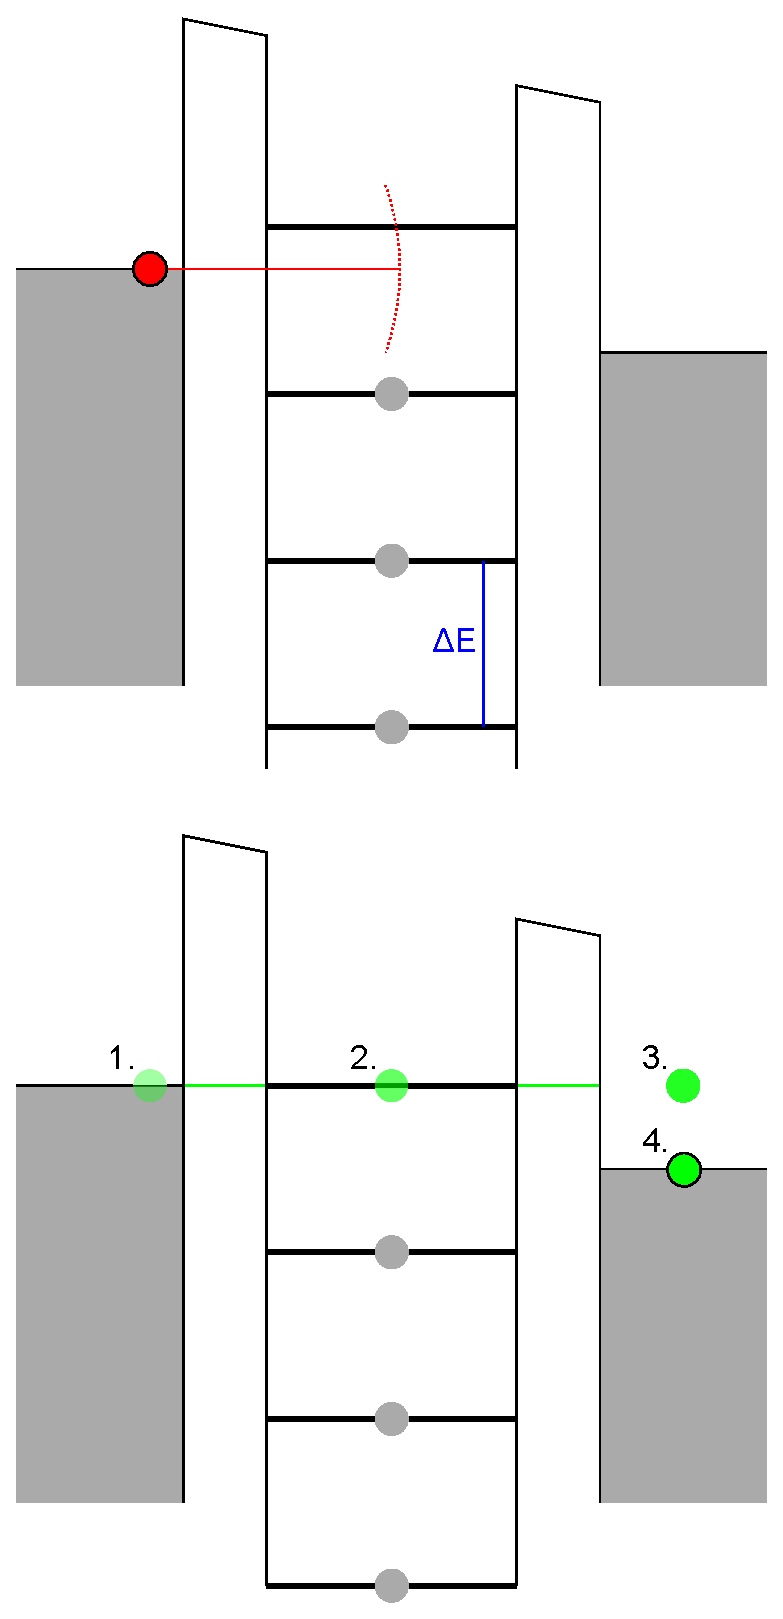
\includegraphics[width=0.6\textwidth, height=0.8\textheight]{coulomb_blockade}
	\caption{A Coulomb Blockade \cite{coulomb_blockade} forms due to electrostatic potential difference between island and source.\\ In the upper diagram, all allowable energy states are below the Fermi energy of the reservoir, hence no transmission can occur.\\ In the lower diagram, the potential of the quantum well has been raised, and now an empty state can be occupied by an electron from the source, which will subsequently tunnel off to the drain.}
	\label{coulomb_blockade}
\end{figure}

\begin{figure}[htbp!]
	\centering
	\includegraphics[width=0.8\textwidth]{coulomb_peaks}
	\caption{Coulomb Peaks form due to the discrete energy levels allowed on the island}
	\label{fig::coulomb_peaks}
\end{figure}



\cite{nuclear_spin_readout}


\cite{bonato2015optimized}
\subsection{Devices}
\subsubsection{PCIe Digitizer Card}
\todo[inline]{Talking points of the Digitizer solution, DMA, etc. etc.}
\cite{ATS9440}
%\subsubsection{FPGA/$\mu$Controller and ADC}
\todo[inline]{Talking points of the external FPGA and ADC solution, mention some particular examples of ADCs etc.}
\subsubsection{XMC}
\todo[inline]{Talking points of the integrated XMC solution, pre-built FPGA, ADCs and possibly with Auto-DMA}

\section{Experimental Design}
With new devices constantly being designed and fabricated, new avenues being probed, the structure of experiments can become convoluted. The needless post-processing of all acquired data to top it all off is \todo[inline]{gargghh}


The apparatus I am applying my work to is by no means comprehensive, but it serves as a reference point in a proven device. To accomplish this body of work with this particular device would 


Figure \ref{fig::set_layout} \cite{morello2010single}
shows the physical device that will be similar to one I will be testing my solution on. This devices has various control points, such as the top gate to induce a layer of electrons on the boundary, the left and right barriers to remove this layer, forming tunnel junctions to the island, and finally the plunger to control the gate, as in a MOSFET.
\subsection{Problem Statement}
\todo[inline]{Say something5}

\begin{figure}[htbp!]
	\centering
	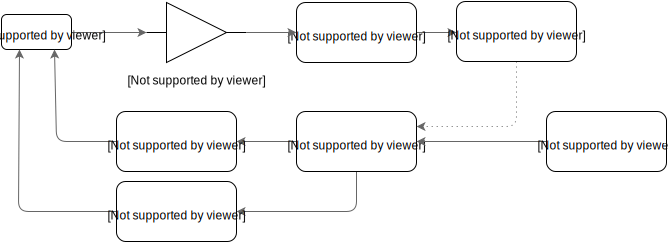
\includegraphics[width=\textwidth]{thesis_experiment.pdf}
	\caption{Block diagram of experiment}
	\label{fig::thesis_experiment}
\end{figure}

\subsection{Digital Devices}
\subsubsection{PCIe Digitizer Card}
\todo[inline]{Talking points of the Digitizer solution, DMA, etc. etc.}
The ATS9440 \gls{pcie} digitizer card \cite{ATS9440} has been incorporated into the previous years' research and hence, a lot of the groundwork has been laid out for using the device, and interfacing it with experiments. It is the natural solution, to attempt to provide digital feedback in a MATLAB environment in a semi-real-time capacity. There is a clear benefit in utilizing what is already well established, conditional that it can achieve what is necessary.

The primary features of this solution are:
\begin{itemize}
	\item Range of sampling frequencies from 1 KS/s to 125 MS/s
	\item 4 independent input channels
	\item Internal (from one of the 4 input channels) and external triggering
	\item 14-bit resolution, with definable input ranges of $\pm 100 \textrm{mV}$ to $\pm 4 \textrm{V}$
	\item Auto-\gls{dma} for fast storage and parallel data processing.
\end{itemize}

\subsubsection{FPGA/$\mu$Controller and ADC}
\todo[inline]{Talking points of the external FPGA and ADC solution, mention some particular examples of ADCs etc.}
An alternative solution is to have an external device which is responsible for detecting peaks in the \gls{set} current, and waiting a predetermined amount of time before setting a TTL output to high, which could then trigger the plunge, and the experiment to begin.

This approach requires the design of a high precision \gls{adc}, with a sampling rate of at least 1 MS/s. The digital data would then need to be processed by either a $\mu$Controller or a \gls{fpga}. The primary benefit of this solution is that it is versatile, and can be adapted and modified to meet different needs of the future. Furthermore, as this is completely external to the rest of the experiment, it can truly run in parallel, and accurate timing without error could prove to be more achievable.
\subsubsection{XMC}
\todo[inline]{Talking points of the integrated XMC solution, pre-built FPGA, ADCs and possibly with Auto-DMA}

\begin{figure}[htbp!]
	\centering
	\includegraphics[width=\textwidth]{set_layout}
	\caption{The layout of an SET}
	\label{fig::set_layout}
\end{figure}
\section{Prospective Plan}
\subsection{Proposed Timeline}
\todo[inline]{A Gantt chart, perhaps with critical tasks highlighted, to be detailed below}
\subsection{Description of Work}
\todo[inline]{Details about what the particulars of work to be done are}
\section{Conclusion}
\todo[inline]{Conclude, like normal}

\bibliographystyle{ieeetr}	%IEEE style referencing
\bibliography{./src/references}

\begin{appendices} 
	\section{Risk Assessment}
	\input{./src/risk_assessment}
	\section{Supplementary Information}
	\paragraph{Big O Notation} describes the limiting behaviour of a function when the argument tends toward infinity.
\label{supp::big_o}
For example, the leading term ($3 x^4$) in the polynomial $p(x) = 3 x^4 + 20 x^2 + 1$, represents the strongest factor that determines the behaviour of the function. As such, we say $p$ has order $\mathcal{O}(n^4)$. Note that we drop any constant multiplier as it doesn't modify the growth or shape of the function.
\end{appendices}
\end{document}
